\chapter{Mezuro: Uma plataforma de Monitoramento de Código Fonte}
\label{cap-mezuro}

No Capítulo \ref{cap-metrics} discutimos as principais questões de \emph{design}, segurança e métricas no contexto da Engenharia de Software. As métricas estáticas de código-fonte são ferramentas que podem ser utilizadas para a compreensão da qualidade e identificação de vulnerabilidades do código-fonte. Entretanto, como discutido no mesmo capítulo, avaliar a qualidade de um software envolve um processo dispendioso e não trivial. Na Seção \ref{sec-metrics-esw}, apresentamos um conjunto de métricas estáticas cujo propósito é mensurar alguns atributos do software tais como complexidade, acoplamento e tamanho. 

%

Entretanto, o esforço necessário para extrair as métricas estáticas manualmente é imensurável, dificultando ainda mais a adoção dessas métricas em projetos de software. Portanto, é de extrema importância a utilização de ferramentas que auxiliem a utilização de métricas de código-fonte, automatizando a extração e visualização dessas métricas. Porém, existem poucas ferramentas disponíveis, e muitas delas nem sempre são adequadas para análise de determinados projetos de software ~\cite{meirelles2010mezuro}. Isso também decorre devido a existência de várias ferramentas extratoras independentes, que seguem seus próprios padrões e oferecem um conjunto de métricas limitados que podem não se adequar para determinados contextos.

%

Em virtude do que foi mencionado foi criado o Mezuro\footnote{\url{http://mezuro.org/}}, uma plataforma livre para monitoramento completo de código-fonte. O Mezuro busca auxiliar em vários problemas relacionados à utilização de métrica, visando ser uma interface que permita, de forma flexível, a extração e análise de métricas estáticas de código-fonte, licensiado como AGPLv3\footnote{\url{http://www.gnu.org/licenses/agpl-3.0.html}} \cite{manzo2014}. O Mezuro é uma plataforma concebida através do amadurecimento de diversas ferramentas, inicializada através do projeto Qualipso\footnote{Quality Platform for Open Source: \url{http://qualipso.icmc.usp.br/}}. Dentre estas ferramentas, destaca-se o Analizo\footnote{\url{http://analizo.org/}}, uma das ferramentas utilizadas pelo Mezuro para extração de métricas de código-fonte em C/C++ e Java.

%

A primeira versão do Mezuro foi criada a partir da plataforma web chamada Noosfero\footnote{\url{http://noosfero.org/}}. O Noosfero é uma plataforma de criação de redes sociais livre, disponível sob licença AGPL\footnote{Licença de software GNU Affero General Public License} V3, que facilita a criação de redes sociais personalizadas e geração de conteúdo colaborativo. O Participa BR \footnote{\url{https://www.participa.br/}}, o Stoa\footnote{\url{http://stoa.usp.br/}} e o Portal da FGA\footnote{\url{http://fga.unb.br/}} são exemplos de portais que utilizam o Noosfero. 

%

O Noosfero é construído em Ruby, implementando a arquitetura MVC através do \emph{framework} Rails. A arquitetura do Noosfero ainda permite a implementação de novas funcionalidades através da criação de \emph{plugins} que podem ser habilitados no ambiente instanciado. Assim, na primeira versão do Mezuro, foi implementado um \emph{plugin} que adicionava as funcionalidades específicas para o monitoramento de código-fonte e realizava a conexão com os outros componentes necessários (explicados a seguir na Seção \ref{sec-mezuro-design}).

%

Entretanto, o Mezuro tem sido evoluído como uma plataforma independente. Isto ocorreu devido à algumas dificuldades existentes inerentes ao acoplamento com o Noosfero, principalmente relacionados às versões das tecnologias ainda utilizadas pelo Noosfero. Além disso, atualmente o Mezuro já possui uma pequena comunidade de colaboradores o que favorece o desacoplamento do código do Mezuro, uma vez que os \emph{plugins} do Noosfero são mantidos junto com o código principal. Com isto, o Mezuro está sendo desenvolvido atualmente com as versões estáveis do Ruby 2\footnote{\url{https://www.ruby-lang.org/}} e Rails 4\footnote{\url{http://rubyonrails.org/}}. A Figura~\ref{mezuro} apresenta a tela principal da nova versão do Mezuro.

%

\graphicspath{{figuras/}}
\begin{figure}[h]
\centering
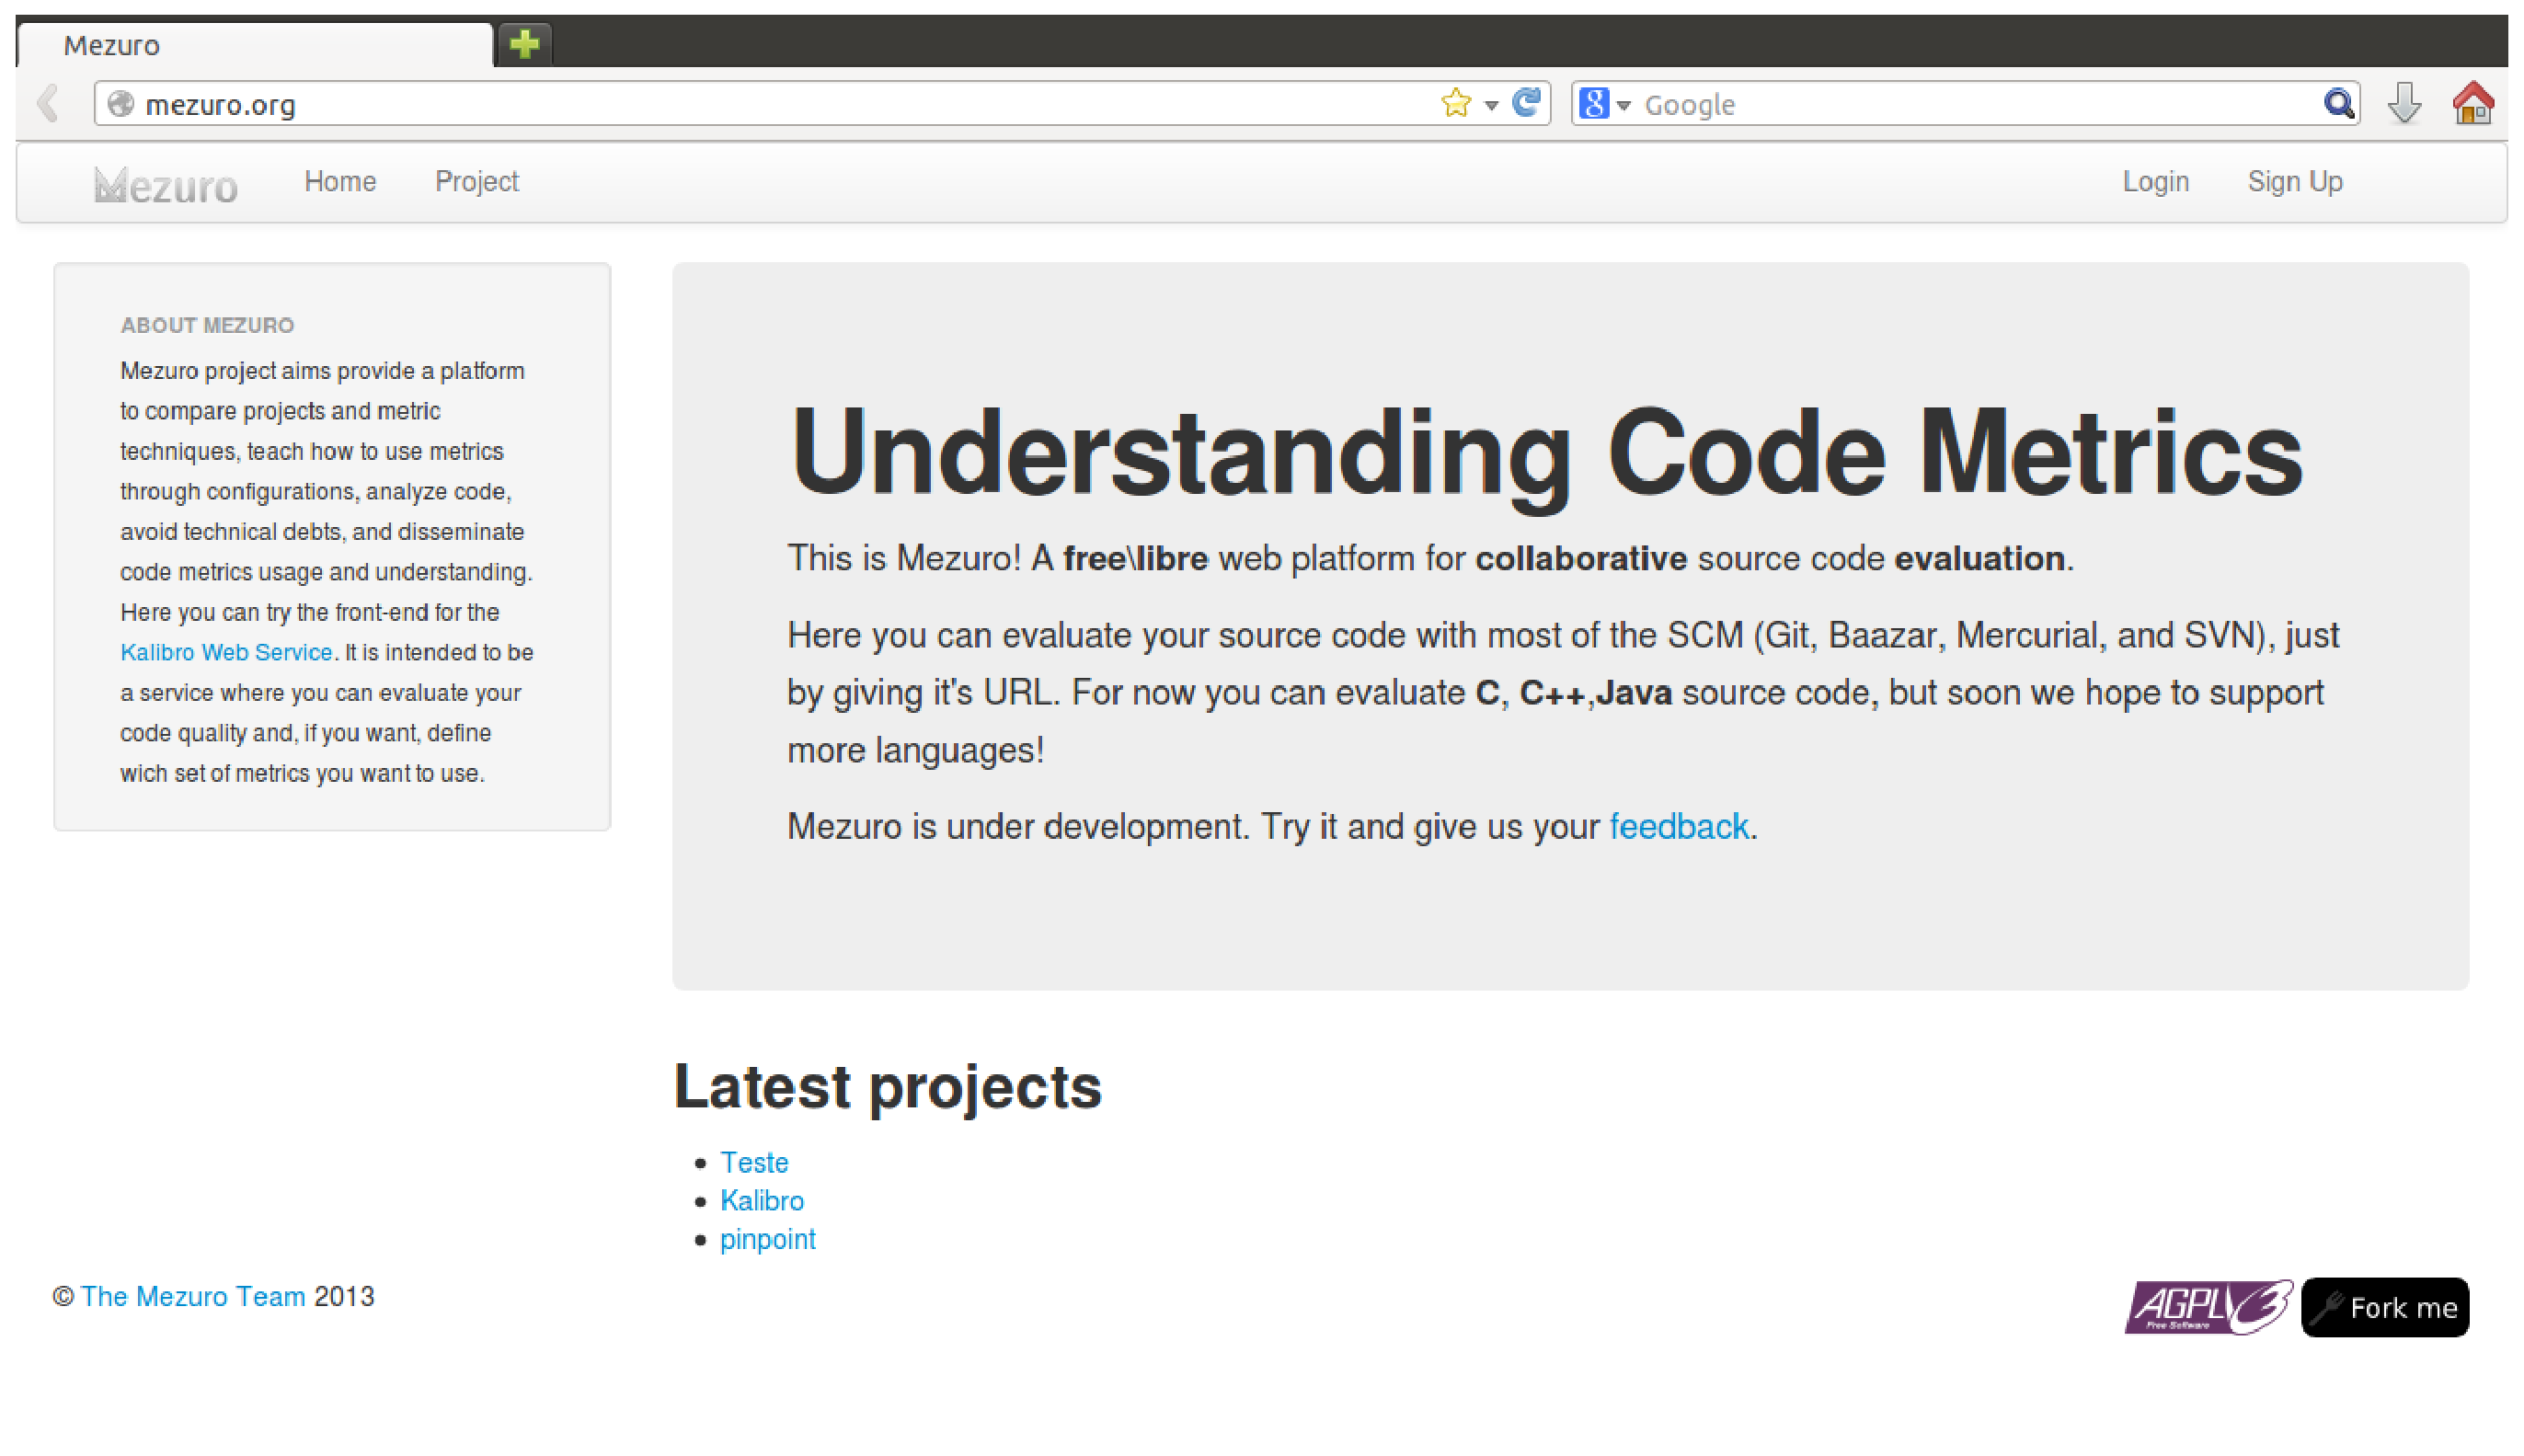
\includegraphics[width=0.7\textwidth]{mezuro-standalone}
\caption{Tela principal do Mezuro. Disponível em \url{http://mezuro.org/}}
\label{mezuro}
\end{figure}

%

Listamos a seguir algumas ferramentas semelhantes ao Mezuro, ferramentas identificadas e detalhadas  através de outros trabalhos \cite{meirelles2010mezuro}\cite{vieira2013}\cite{manzo2014}:

%

\begin{itemize}
\item \textbf{SonarQube}\footnote{\url{http://www.sonarqube.org/}} - Plataforma livre de gerenciamento de qualidade de código que classifica problemas encontrados e calcula métricas simples relacionados a testes e dívidas técnicas.
\item \textbf{CodeClimate}\footnote{\url{https://codeclimate.com/}} - Ferramenta que procura identificar \emph{code smells} no software em análise e classificá-los a partir de notas que varia de \emph{A} a \emph{F}. Esta ferramenta fornece análise sobre códigos JavaScript e Ruby.
\item \textbf{SQO-OSS}\footnote{\url{http://www.sqo-oss.org/}} (\emph{Software Quality Assessment of Open Source Software}) - Conjunto de ferramentas de análise e \emph{benchmarking} de projetos de software livre.
\end{itemize}

%

Destacamos as principais características do Mezuro, que também serão discutidas durante a apresentação da arquitetura da ferramenta:

%

\begin{itemize}
\item Coletar dados a partir de diversos extratores, possibilitando a escolha  rica de diversas métricas. Além disso, o Mezuro é extensível para a inserção de extratores diferentes.
\item Criação de configurações que são um conjunto de métricas e parâmetros que podem ser utilizadas para a avaliação de um projeto. Esta característica permite que especialistas definam os parâmetros e métricas adequadas para um determinado contexto, sendo que uma configuração também pode ser aplicado em outros projetos a depender da necessidade de quem utilizará a ferramenta.
\item Criação de intervalos qualitativos associado a valores de métricas. Esta característica é muito importante para a utilização das métricas, uma vez que abstraem a interpretação direta dos valores obtidos para definições mais simples como bom, regular e ruim.
\item Criação de métricas mais complexas a partir da combinação de métricas nativas, flexibilizando e estendendo a utilização da ferramenta.
\item Monitoramento de projetos a partir de repositórios ou arquivos compactados. As opções de repositórios possíveis incluem o GIT, Subversion e o Bazaar. Vale ressaltar que os resultados dos monitoramentos são públicos a acessíveis à comunidade.
\item Monitoramento de projetos com periodicidade definido pelo usuário.
\item Escolha de qual configuração um determinado projeto irá utilizar.
\end{itemize}

%

\section{Arquitetura do Mezuro}
\label{sec-mezuro-design}

Como mencionado, o Mezuro está evoluindo para uma aplicação independente. Neste sentido, a arquitetura da plataforma como um todo está sendo modificada, visando principalmente maior modularização em diversos serviços independentes. A Figura~\ref{fig:mezuro-current-design} apresenta a arquitetura atual da plataforma.

% \graphicspath{{figuras/}}
% \begin{figure}[h]
% \centering
% 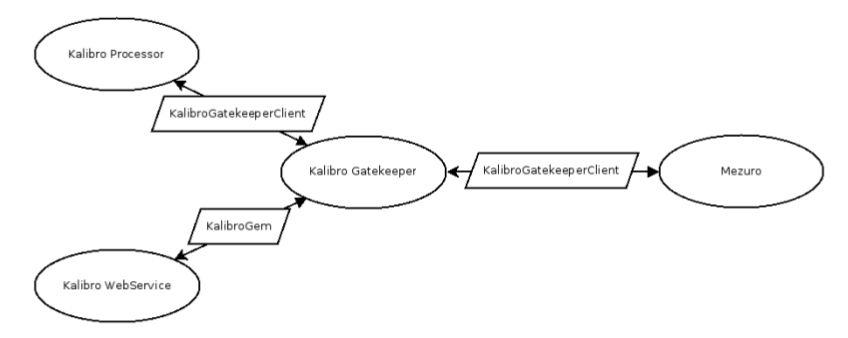
\includegraphics[width=0.6\textwidth]{MezuroAtual.png}
% \caption{Arquitetura Atual do Mezuro. Extraído de \cite{manzo2014}}
% \label{fig:mezuro-current-design}
% \end{figure}

%

O Mezuro utiliza o WebService Kalibro Metrics~\footnote{\url{http://kalibro.org}} para fornecer a funcionalidade de análise e avaliação de métricas de código-fonte. O Kalibro é um WebService SOAP\footnote{Simple Object Access Protocol}, baseado em mensagens XML\footnote{Linguagem de Marcação Extensível} cujos componentes correspondem Kalibro WebService. O principal objetivo do Kalibro é se conectar com ferramentas extratoras de métricas, como o Analizo, executando-as para realizar a coleta de dados. Outro módulo é representado pela elipse Kalibro Processor cujo objetivo é centralizar o processamento de métricas. Por último, a comunicação entre todos estes módulos principais é intermediada pelo módulo correspondente à elipse Kalibro Gatekeeper.

%

Dentre os objetivos da evolução desta arquitetura, tem-se a reescrita do Kalibro e sua modularização em três serviços principais, que pode ser observada na Figura~\ref{fig:mezuro-future-design}. O primeiro módulo já está em uso, sendo também represetado na Figura~\ref{fig:mezuro-current-design}, é o módulo Kalibro Processor. Neste sentido, a contemplação desta nova arquitetura consiste na reescrita de serviços do Kalibro, de Java para Ruby, para concepção de dois novos módulos: Kalibro Project e Kalibro Configuration, responsáveis pelo processamento de projetos e configuração respectivamente. Esta nova proposta apoia a modularização e o baixo acoplamento, utilizando-se principalmente o conceito de orquestração de serviços que podem ser encontrados em Arquiteturas Orientadas à Serviço - SOA \cite{thomaserl2007}.

% \graphicspath{{figuras/}}
% \begin{figure}[h]
% \centering
% 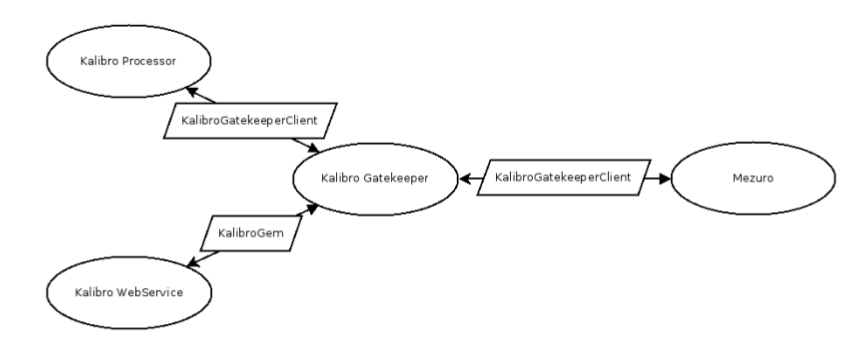
\includegraphics[width=0.6\textwidth]{MezuroNovo.png}
% \caption{Arquitetura Futura do Mezuro. Extraído de \cite{manzo2014}}
% \label{fig:mezuro-future-design}
% \end{figure}

%

\section{Evolução do Mezuro}

Um dos principais objetivos desta monografia é utilizar a platarforma Mezuro para contemplar algumas das questões de pesquisa deste trabalho. Assim, o Mezuro será utilizado como proposta para avaliar o uso de uma plataforma de monitoramento de código-fonte em projetos de software. 

%

Atualmente, a evolução do Mezuro está no ponto de finalização do módulo Kalibro Processor. Portanto, pretendemos contribuir para com a evolução do Mezuro como plataforma independente em diferentes níveis. Dada os objetivos tecnológicos e de pequisa expostos no Capítulo \ref{cap-introducao}, essas contribuições devem ser realizadas nos diferentes módulos apresentados na Figura~\ref{fig:mezuro-future-design}, contemplando a inserção de novos extratores e métricas sob o Kalibro, assim como melhorias relacionadas as formas de acompanhamento e configuração de métricas.

%

Estas contribuições serão de suma importância para esta monografia, assim como para a evolução do Mezuro, uma vez que as decisões serão compartilhadas com a comunidade de desenvolvedores e as contribuições em código terão impactos importantes e comuns quando se trata de software livre. Portanto, as contribuições irão ajudar para melhor compreensão da utilização do Mezuro e suas funcionalidades. Além disso, algumas das evoluções desejadas e destacadas no Capítulo \ref{cap-introducao} podem se tornar fundamentais para que o Mezuro possa se tornar não só uma ferramenta com viés acadêmico, mas que também contemple diferentes objetivos dentro de projetos de software. Pretende-se ainda adicionar novos extratores e métricas ao Mezuro, o torando ainda mais flexível e aumentando seu potencial de uso.

%

Por fim, vale ressaltar que, dado o contexto desta monografia, a contribuição com o software livre Mezuro é uma excelente oportunidade de se exercitar os principais conhecimentos obtidos ao longo do curso de Engenharia de Software.

%


